\documentclass[a4paper,12pt]{report}
\usepackage{mathtext}
\usepackage[T2A]{fontenc}
\usepackage[utf8]{inputenc}
\usepackage[english,russian]{babel}
\usepackage{geometry}
\usepackage{listings}
\usepackage{amsmath}
\geometry{top=2cm}
\usepackage{titlesec}
\usepackage{color}
\usepackage{pgfplots}
\usepackage{filecontents}
\usetikzlibrary{datavisualization}
\usetikzlibrary{datavisualization.formats.functions}
\usepackage{caption}
\DeclareCaptionFont{white}{\color{white}}
\DeclareCaptionFormat{listing}{\colorbox{gray}{\parbox{\textwidth}{#1#2#3}}}
\captionsetup[lstlisting]{format=listing,labelfont=white,textfont=white}

% Для листинга кода:
\lstset{ %
language=C++,                 % выбор языка для подсветки
basicstyle=\small\sffamily, % размер и начертание шрифта для подсветки кода
numbers=left,               % где поставить нумерацию строк (слева\справа)
numberstyle=\tiny,           % размер шрифта для номеров строк
stepnumber=1,                   % размер шага между двумя номерами строк
numbersep=-5pt,                % как далеко отстоят номера строк от подсвечиваемого кода
showspaces=false,
backgroundcolor=\color{white},         
showstringspaces=false,      % показывать или нет пробелы в строках
showtabs=false,             % показывать или нет табуляцию в строках
frame=single,              % рисовать рамку вокруг кода
tabsize=2,                 % размер табуляции по умолчанию равен 2 пробелам
captionpos=t,              % позиция заголовка вверху [t] или внизу [b] 
breaklines=true,           % автоматически переносить строки (да\нет)
breakatwhitespace=false, % переносить строки только если есть пробел
escapeinside={\%*}{*)},   % если нужно добавить комментарии в коде
	    keywordstyle=\color{blue}\ttfamily,
	    stringstyle=\color{red}\ttfamily,
	    commentstyle=\color{green}\ttfamily,
	    morecomment=[l][\color{magenta}]{\#},
	    columns=fullflexible   % если нужно добавить комментарии в коде
}

% Для измененных титулов глав:
\definecolor{gray75}{gray}{0.75} % определяем цвет
\newcommand{\hsp}{\hspace{20pt}} % длина линии в 20pt
% titleformat определяет стиль
\titleformat{\chapter}[hang]{\Huge\bfseries}{\thechapter\hsp\textcolor{gray75}{|}\hsp}{0pt}{\Huge\bfseries}


% Графики
\begin{filecontents}{VinogradEven.dat}
100
200
300
400
500
600
700
800
900
1000
\end{filecontents}

\begin{filecontents}{x2ThreadedEven.dat}
100
200
300
400
500
600
700
800
900
1000
\end{filecontents}

\begin{filecontents}{x4ThreadedEven.dat}
100
200
300
400
500
600
700
800
900
1000
\end{filecontents}

\begin{filecontents}{x8ThreadedEven.dat}
100
200
300
400
500
600
700
800
900
1000
\end{filecontents}

\begin{filecontents}{VinogradOdd.dat}
100
200
300
400
500
600
700
800
900
1000
\end{filecontents}

\begin{filecontents}{x2ThreadedOdd.dat}
100
200
300
400
500
600
700
800
900
1000
\end{filecontents}

\begin{filecontents}{x4ThreadedOdd.dat}
100
200
300
400
500
600
700
800
900
1000
\end{filecontents}

\begin{filecontents}{x8ThreadedOdd.dat}
100
200
300
400
500
600
700
800
900
1000
\end{filecontents}


\begin{document}
\begin{titlepage}
	\centering
	{\scshape\LARGE МГТУ им. Баумана \par}
	\vspace{4cm}
	{\scshape\Large Лабораторная работа №2\par}
	\vspace{0.5cm}	
	{\scshape\Large По курсу: "Анализ алгоритмов"\par}
	\vspace{2cm}
	{\huge\bfseries Параллельное умножение матриц\par}
	\vspace{3cm}
	\Large Работу выполнил: Луговой Дмитрий, ИУ7-51Б\par
	\vspace{0.5cm}
	\Large Преподаватель:  Волкова Л.Л.\par

	\vfill
	\large \textit {Москва, 2019} \par
\end{titlepage}

\setcounter{page}{2}

\tableofcontents

\newpage
\chapter*{Введение}
\addcontentsline{toc}{chapter}{Введение}
\hspace{0.6cm} \textbf{Цель работы}: изучение возможности параллельных вычислений и использование такого подхода на практике. Реализация парралельного алгоритма Винограда умножения матриц. 
В данной лабораторной работе рассматривается алгоритм Винограда и параллельный алгоритм Винограда. Необходимо сравнить зависимость времени работы алгоритма от числа параллельных потоков и размера матриц, провести сравнение стандартного и параллельного алгоритмов.

\textbf{\LARGE Задачи работы}\\\\
Задачами данной лабораторной являются:
\begin{enumerate}
\item[1)] Научиться писать многопоточные программы;
\item[2)] Применить полученные знания на практике, переписав алгоритм Винограда в несколько потоков;
\item[3)] Провести замеры скорости работы однопоточной и многопоточной реализаций и проанализировать полученные результаты.
\end{enumerate}


\chapter{Аналитическая часть}
\hspace{0.6cm}В данном разделе содержатся описание алгоритма Винограда умножения матриц, определение потока и многопоточного программирования.

\section{Стандартный алгоритм}
\hspace{0.6cm}Пусть даны две прямоугольные матрицы A и B размерностей $m \times n$ , $n \times q$ соответственно:

\[
A = 
  \begin{bmatrix} 
    a_{11} & a_{12} & \cdots & a_{1n} \\
    a_{21} & a_{22} & \cdots & a_{2n} \\ 
    \vdots & \vdots & \ddots & \vdots \\ 
    a_{m1} & a_{m2} & \cdots & a_{mn}
  \end{bmatrix},\;\;\;
\]
\[
B =   
  \begin{bmatrix} 
    b_{11} & b_{12} & \cdots & b_{1q} \\
    b_{21} & b_{22} & \cdots & b_{2q} \\ 
    \vdots & \vdots & \ddots & \vdots \\ 
    b_{n1} & b_{n2} & \cdots & b_{nq}.
  \end{bmatrix}.
\]
Тогда матрица C размерностью $m \times q$
\[
C = 
  \begin{bmatrix} 
    c_{11} & c_{12} & \cdots & c_{1q} \\
    c_{21} & c_{22} & \cdots & c_{2q} \\ 
    \vdots & \vdots & \ddots & \vdots \\ 
    c_{m1} & c_{m2} & \cdots & c_{mq}
  \end{bmatrix},
\]
в которой:\\

$c_{ij} = \sum_{k=1}^n a_{ik}b_{kj} \;\;\; \left(i=1, 2, \ldots m;\; j=1, 2, \ldots q \right)$\\

называется их произведением. Операция умножения двух матриц выполнима только в том случае, если число столбцов в первом сомножителе равно числу строк во втором; в этом случае говорят, что матрицы согласованы. В частности, умножение всегда выполнимо, если оба сомножителя — [[Квадратная матрица|квадратная матрица]] одного и того же порядка. 

Таким образом, из существования произведения AB вовсе не следует существование произведения BA

\section{Алгоритм Винограда}
\hspace{0.6cm} \textbf {АлгоритмВинограда} — алгоритм умножения матриц, предложенный в 1987 году Д. Копперсмитом и Ш. Виноградом. В исходной версии асимптотическая сложность алгоритма составляла $O(n^{2,3755})$, где n — размер стороны матрицы. Алгоритм Копперсмита—Винограда, с учетом серии улучшений и доработок в последующие годы, обладает лучшей асимптотикой среди известных алгоритмов умножения матриц.\\
Если посмотреть на результат умножения двух матриц, то видно, что каждый элемент в нем представляет собой скалярное произведение соответствующих строки и столбца исходных матриц. Можно заметить также, что такое умножение допускает предварительную обработку, позволяющую часть работы выполнить заранее. 
Рассмотрим два вектора
$V = (v1, v2, v3, v4)$ и
$W = (w1, w2, w3, w4)$.
Их скалярное произведение равно: 
$V * W = v1w1 + v2w2 + v3w3 + v4w4$.
Это равенство можно переписать в виде: 
$V * W = (v1 + w2)(v2 + w1) + (v3 + w4)(v4 + w3) - v1v2 - v3v4 - w1w2 - w3w4$.

Кажется, что второе выражение задает больше работы, чем первое: вместо четырех умножений мы насчитываем их шесть, а вместо трех сложений - десять. Однако выражение в правой части последнего равенства допускает предварительную обработку: его части можно вычислить заранее и запомнить для каждой строки первой матрицы и для каждого столбца второй. На практике это означает, что над предварительно обработанными элементами нам придется выполнять лишь первые два умножения и последующие пять сложений, а также дополнительно два сложения.

\section{Многопоточность}
\hspace{0.6cm} \textbf {Поток выполнения} — наименьшая единица обработки, исполнение которой может быть назначено ядром операционной системы. Реализация потоков выполнения и процессов в разных операционных системах отличается друг от друга, но в большинстве случаев поток выполнения находится внутри процесса. Несколько потоков выполнения могут существовать в рамках одного и того же процесса и совместно использовать ресурсы, такие как память, тогда как процессы не разделяют этих ресурсов. В частности, потоки выполнения разделяют инструкции процесса (его код) и его контекст (значения переменных, которые они имеют в любой момент времени).

На одном процессоре многопоточность обычно происходит путём временного мультиплексирования (как и в случае многозадачности): процессор переключается между разными потоками выполнения. Это переключение контекста обычно происходит достаточно часто, чтобы пользователь воспринимал выполнение потоков или задач как одновременное. В многопроцессорных и многоядерных системах потоки или задачи могут реально выполняться одновременно, при этом каждый процессор или ядро обрабатывает отдельный поток или задачу.

Потоки возникли в операционных системах как средство распараллеливания вычислений.

Параллельное выполнение нескольких работ в рамках одного интерактивного приложения повышает эффективность работы пользователя. Так, при работе с текстовым редактором желательно иметь возможность совмещать набор нового текста с такими продолжительными по времени операциями, как переформатирование значительной части текста, печать документа или его сохранение на локальном или удаленном диске. Еще одним примером необходимости распараллеливания является сетевой сервер баз данных. В этом случае параллелизм желателен как для обслуживания различных запросов к базе данных, так и для более быстрого выполнения отдельного запроса за счет одновременного просмотра различных записей базы. Именно для этих целей современные ОС предлагают механизм многопоточной обработки (multithreading). Понятию «поток» соответствует последовательный переход процессора от одной команды программы к другой. ОС распределяет процессорное время между потоками. Процессу ОС назначает адресное пространство и набор ресурсов, которые совместно используются всеми его потоками \cite{multithreading_history}.

Создание потоков требует от ОС меньших накладных расходов, чем процессов. В отличие от процессов, которые принадлежат разным, вообще говоря, конкурирующим приложениям, все потоки одного процесса всегда принадлежат одному приложению, поэтому ОС изолирует потоки в гораздо меньшей степени, нежели процессы в традиционной мультипрограммной системе. Все потоки одного процесса используют общие файлы, таймеры, устройства, одну и ту же область оперативной памяти, одно и то же адресное пространство. Это означает, что они разделяют одни и те же глобальные переменные. Поскольку каждый поток может иметь доступ к любому виртуальному адресу процесса, один поток может использовать стек другого потока. Между потоками одного процесса нет полной защиты, потому что, во-первых, это невозможно, а во-вторых, не нужно. Чтобы организовать взаимодействие и обмен данными, потокам вовсе не требуется обращаться к ОС, им достаточно использовать общую память — один поток записывает данные, а другой читает их. С другой стороны, потоки разных процессов по-прежнему хорошо защищены друг от друга.

\chapter{Конструкторская часть}
\hspace{0.6cm}В этом разделе содержится cхема алгоритма Винограда умножения матриц и описание распараллеливания этого алгоритма.
\newpage
\section{Схемы алгоритмов}

\hspace{0.6cm}На Рис.2.1 и 2.2 представлена схема стандартного алгоритма умножения матриц.
\begin{figure}[ht!]
\center{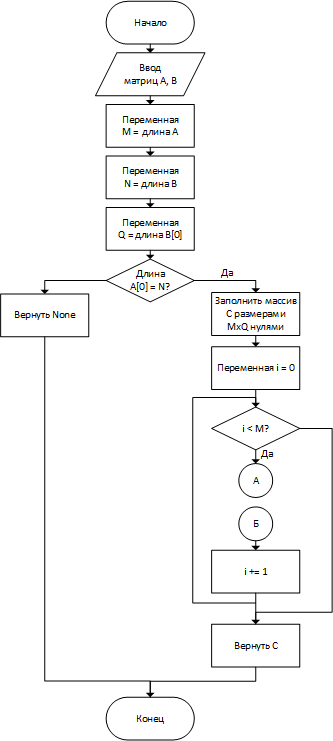
\includegraphics[scale=1]{Standart1.png}}
\caption{Стандартный алгоритм умножения матриц}
\newpage
\end{figure}
\newpage
\begin{figure}[ht!]
\center{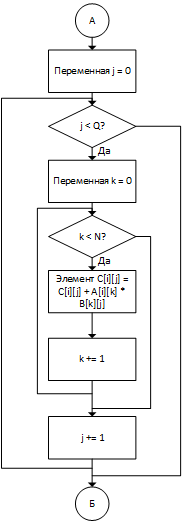
\includegraphics[scale=1]{Standart2.png}}
\caption{Стандартный алгоритм умножения матриц(продолжение)}
\end{figure}
\newpage
На Рис.2.3, 2.4, 2.5 и 2.6 представлена схема алгоритма Винограда умножения матриц.
\begin{figure}[ht!]
\center{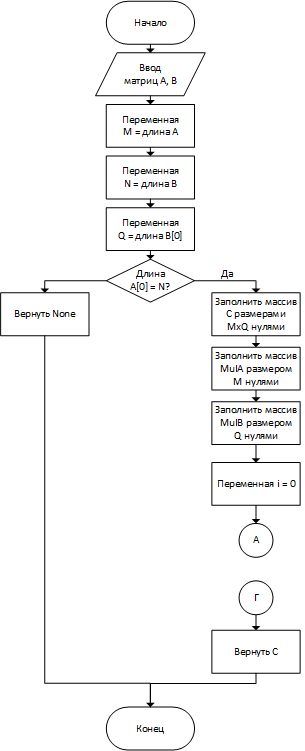
\includegraphics[scale=1]{Vinograd1.png}}
\caption{Алгоритм Винограда умножения матриц}
\end{figure}
\newpage
\begin{figure}[ht!]
\center{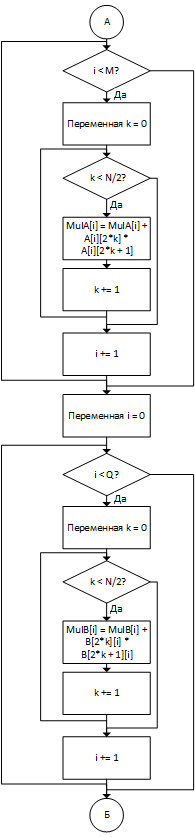
\includegraphics[scale=1]{Vinograd2.png}}
\caption{Алгоритм Винограда умножения матриц(продолжение 1)}
\end{figure}
\newpage
\begin{figure}[ht!]
\center{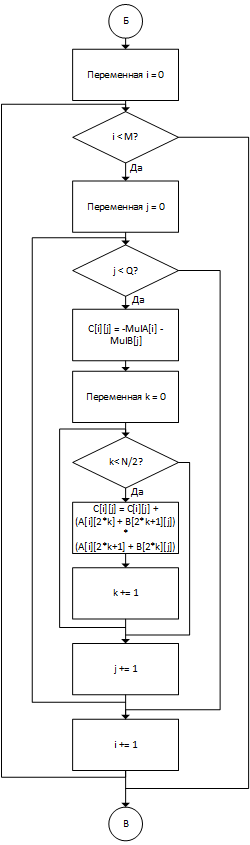
\includegraphics[scale=1]{Vinograd3.png}}
\caption{Алгоритм Винограда умножения матриц(продолжение 2)}
\end{figure}
\newpage
\begin{figure}[ht!]
\center{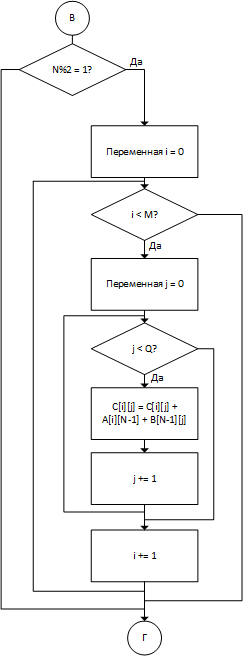
\includegraphics[scale=1]{Vinograd4.png}}
\caption{Алгоритм Винограда умножения матриц(продолжение 3)}
\end{figure}
\newpage

На Рис.2.7, 2.8, 2.9 и 2.10 представлена схема оптимизированного алгоритма Винограда умножения матриц.

\begin{figure}[ht!]
\center{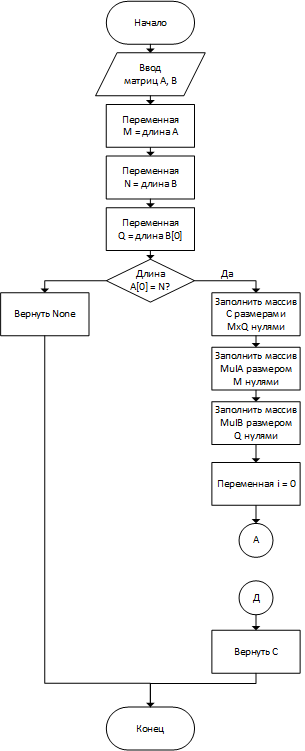
\includegraphics[scale=1]{Optimized1.png}}
\caption{Оптимизированный алгоритм Винограда умножения матриц}
\end{figure}

\newpage

\begin{figure}[ht!]
\center{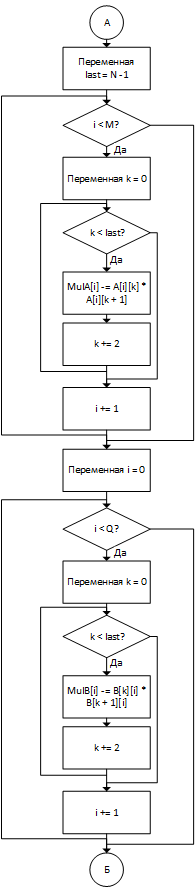
\includegraphics[scale=0.9]{Optimized2.png}}
\caption{Оптимизированный алгоритм Винограда умножения матриц(продолжение 1)}
\end{figure}

\newpage

\begin{figure}[ht!]
\center{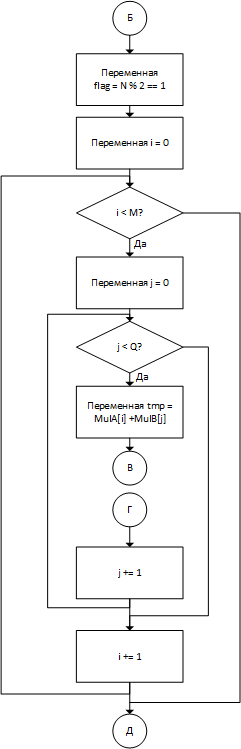
\includegraphics[scale=1]{Optimized3.png}}
\caption{Оптимизированный алгоритм Винограда умножения матриц(продолжение 2)}
\end{figure}

\newpage

\begin{figure}[ht!]
\center{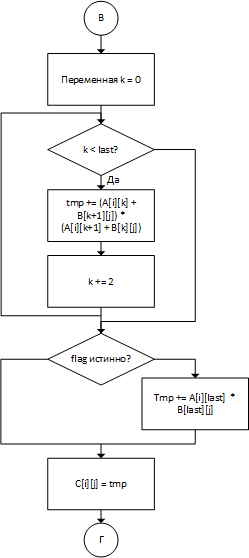
\includegraphics[scale=1]{Optimized4.png}}
\caption{Оптимизированный алгоритм Винограда умножения матриц(продолжение 3)}
\end{figure}

\newpage

\section{Расчет трудоемкости}

\hspace{0.6cm}Пусть заданы матрицы размерами $m \times n$ , $n \times q$. Используя модель вычислений, заданную ранее, произведем подсчет трудоемкости алгоритмов умножения матриц:
\begin{itemize}

\item Стандартный алгоритм
\[
f_{стд} = 2 + M(2 + 2 + Q(2 + 2 + N(2 + 8 + 1 + 1 + 1))) = 13MNQ + 4MQ + 4M + 2 \approx 13MNQ 
\]

\item Алгоритм Винограда
\begin{align*}
& f_{I} = 2 + M(2 + 3 + \frac{N}{2} (3 + 1 + 6 + 2 + 3)) = \frac{15}{2} MN + 5M + 2\\
& f_{II} = 2 + Q(2 + 3 + \frac{N}{2} (3 + 1 + 6 + 2 + 3)) = \frac{15}{2} QN + 5Q + 2\\
& f_{III} = 2 + M(2 + 2 + Q(2 + 7 + 3 + \frac{N}{2}(3 + 6 + 17))) = 13MNQ + 12 MQ + 4M + 2\\
& f_{IV} = 2 + \left[
	\begin{array}{ccc}
     0, & N \ четное \\
     12MQ + 4M + 2,  & N \ нечетное \\
  \end{array}
  \right.\\
\end{align*}
\begin{multline*} 
f_{вин} = f_{I} + f_{II} + f_{III} + f_{IV} = \frac{15}{2} MN + \frac{15}{2} QN + 9M + 8 + 5Q \\ + 13MNQ + 12MQ + \left[
	\begin{array}{ccc}
     0, & N \ четное \\
     12MQ + 4M + 2,  & N \ нечетное \\
  \end{array}
  \right. \approx 13MNQ
\end{multline*}

\item Оптимизированный алгоритм Винограда
\begin{align*}
& f_{I}^{*} = 2 + M(2 + 2 + \frac{N}{2} (2 + 1 + 5 + 1 + 1)) =  5MN + 4M + 2\\
& f_{II}^{*} =  2 + Q(2 + 2 + \frac{N}{2} (2 + 1 + 5 + 1 + 1)) =  5QN + 4Q + 2\\
& f_{III}^{*} = 5 + 2 + M(2 + 2 + Q(2 + 4 + 2 + \frac{N}{2}(2 + 14) + 1 + 3 + \left[
	\begin{array}{ccc}
     0, & N \ четное \\
     6,  & N \ нечетное \\
  \end{array}
  \right.)) = \\ 
  & = 7 + 4M + 12MQ + 8MNQ + \left[
	\begin{array}{ccc}
     0, & N \ четное \\
     6MQ,  & N \ нечетное \\
  \end{array}
  \right.
\end{align*}
\begin{multline*} 
f_{вин}^{*} = f_{I}^{*} + f_{II}^{*} + f_{III}^{*} = 5MN + 8M + 11 + \\5QN + 4Q + 12MQ + 8MNQ + \left[
	\begin{array}{ccc}
     0, & N \ четное \\
     6MQ,  & N \ нечетное \\
  \end{array}
  \right. \approx 8MNQ
\end{multline*}
\end{itemize}

Как видно из вычислений, наиболее эффективным по трудоемкости является оптимизированный алгоритм Винограда. 
\newpage
Трудоемкость удалось снизить за счет следующих оптимизаций:
\begin{enumerate}
\item Замена $C[i][j] = C[i][j] + \ldots$ на $C[i][j] \text{+=} \ldots$
\item Замена цикла по $k$ от $0$ до $N/2$ с шагом $1$ на цикл от $0$ до $N$ с шагом $2$, что убрало лишние умножения на 2
\item Элементы $MulA$ и $MulB$ сразу высчитываются отрицательными, что убирает 1 операцию отрицания в цикле
\item Замена $C[i][j] = \ldots$ в цикле по $k$ на буферную переменную, что убирает 2 операции индлексирования во внутреннем цикле, но добавляет С[i][j] = tmp во внешний цикл
\item Перенос проверки четности внутрь основного цикла, что ухудшило лучший случай, но улучшило худший
\item Вычисление условия четности и значения $N-1$, тем самым улучшая и лучший, и худший случаи
\end{enumerate}
\chapter{Технологическая часть}
\hspace{0.6cm}В данном разделе приведены требования к программнму обеспечению, средства реализации и листинги кода
\section{Требования к ПО}

\hspace{0.6cm}На вход поступают две целочисленные матрицы, на выходе должен возвращаться результат их умножения, либо сообщение о невозможности их умножения.
	

\section{Средства реализации}
\hspace{0.6cm}Для реализации представленных алгоритмов был выбран язык Python. Время работы алгоритмов было замерено с помощью функции process\_time() из библиотеки time.

\section{Листинги кода}

\hspace{0.6cm}В Листинге 3.1 показана реализация стандартного алгоритма умножения матриц.

\begin{lstlisting}[caption=Функция стандартного умножения матриц]
  def standard_multiply(a, b):
      m = len(a)
      n = len(b)
      if m == 0 or n == 0 or len(a[0]) != n:
          return None
      q = len(b[0])
      c = [[0 for i in range(q)] for j in range(m)]
      for i in range(m):
          for j in range(q):
              for k in range(n):
                  c[i][j] = c[i][j] + a[i][k] * b[k][j]
      return c
\end{lstlisting}
\newpage
В Листинге 3.2 показана реализация алгоритма Винограда умножения матриц.
\begin{lstlisting}[caption=Функция умножения матриц алгоритмом Винограда]
  def vinograd_multiply(a, b):
      m = len(a)
      n = len(b)
      if m == 0 or n == 0 or len(a[0]) != n:
          return None
      q = len(b[0])
      # Part I
      r = n // 2
      mul_a = [0] * m
      for i in range(m):
          for j in range(r):
              mul_a[i] = mul_a[i] + a[i][j * 2] * a[i][j * 2 + 1]

      # Part II
      mul_b = [0] * q
      for i in range(q):
          for j in range(r):
              mul_b[i] = mul_b[i] + b[j * 2][i] * b[j * 2 + 1][i]

      # Part III
      c = [[0 for i in range(q)] for j in range(m)]
      for i in range(m):
          for j in range(q):
              c[i][j] = -mul_a[i] - mul_b[j]
              for k in range(r):
                  c[i][j] = c[i][j] + (a[i][2 * k] + b[2 * k + 1][j]) \
                            * (a[i][2 * k + 1] + b[2 * k][j])

      # Part IV
      if n % 2 == 1:
          for i in range(m):
              for j in range(q):
                  c[i][j] = c[i][j] + a[i][n - 1] * b[n - 1][j]
      return c
\end{lstlisting}
\newpage
В Листинге 3.3 показана реализация оптимизированного алгоритма Винограда умножения матриц.
\begin{lstlisting}[caption=Функция умножения матриц оптимизированным алгоритмом Винограда]
  def optimized_vinograd_multiply(a, b):
      m = len(a)
      n = len(b)
      if m == 0 or n == 0 or len(a[0]) != n:
          return None
      q = len(b[0])
      last = n - 1  # Optimization for odd numbers
      # Part I
      mul_a = [0] * m
      for i in range(m):
          for j in range(0, last, 2):  # Optimization for n // 2
              mul_a[i] -= a[i][j] * a[i][j + 1]  # Optimization for negative and +=

      # Part II
      mul_b = [0] * q
      for i in range(q):
          for j in range(0, last, 2):  # Optimization for n // 2
              mul_b[i] -= b[j][i] * b[j + 1][i]  # Optimization for negative and +=

      flag = n % 2 == 1
      # Part III
      c = [[0 for i in range(q)] for j in range(m)]
      for i in range(m):
          for j in range(q):
              tmp = mul_a[i] + mul_b[j]  # Optimization for buffer
              for k in range(0, last, 2):  # Optimization for n // 2
                  tmp += (a[i][k] + b[k + 1][j]) \
                         * (a[i][k + 1] + b[k][j])  # Optimization for +=
              if flag:  # Optimization for odd numbers
                  tmp += a[i][last] * b[last][j]
              c[i][j] = tmp

      return c
\end{lstlisting}



\chapter{Экспериментальная часть}
В данном разделе приведены примеры работы программы, постановка эксперимента и сравнительный анализ алгоритмов на основе экспериментальных данных.
\section{Примеры работы}
\hspace{0.6cm}\textbf {Пример 1}\\
Матрица A:\\
1 2 3\\
4 5 6\\
Матрица B:\\
1\\
2\\
3\\
Результирующая матрица:\\
14\\
32\\

\textbf {Пример 2}\\
Матрица A:\\
5 2\\
1 4\\
Матрица B:\\\
0 3\\
-6 1\\
Результирующая матрица:\\
-12 17\\
-24 7\\

\newpage 
\textbf {Пример 3}\\
Матрица A:\\
2 7\\
1 3\\
Матрица B:\\
-3 7\\
1 -2\\
Результирующая матрица:\\
1 0\\
0 1\\

\section{Функциональное тестирование}
\hspace{0.6cm}Было проведено функциональное тестирование программы, результаты которого занесены в Таблицу 4.1,1 столбец которой - номер тестового случая, 2 и 3 столбцы - виды матриц, поступающих на вход, 4 столбец - ожидаемый результат, где $None$ означает, что матрицы несовместимы по размеру, 5 столбец - полученный результат. \\

\begin{table}[h!]
\begin{center}
\begin{tabular}{| c | c | c | c | c |}
\hline
№ & A & B & Ожидаемый результат & Полученный результат \\
\hline
1 & Случайная & Пустая & None & None\\
\hline
2 & Пустая & Случайная & None & None\\
\hline
3 & Пустая & Пустая & None & None\\
\hline
4 & Случайная & Нулевая & Нулевая & Нулевая\\
\hline
5 & Нулевая & Случайная & Нулевая  & Нулевая \\
\hline
6 & Единичная & Квадратная & B & B\\
\hline
7 & Квадратная & Единичная & A & A\\
\hline
8 & Размера $M \times N$ & Размера $M \times N$ & None & None\\
\hline
\end{tabular}
\caption{Тестовые случаи}
\end{center}
\end{table}

Программа успешно прошла все тестовые случаи, все полученные результаты совпали с ожидаемыми.

\section{Сравение алгоритмов по времени}
\hspace{0.6cm}Для экспериментов использовались матрицы, размер которых варьируется от $100 \times 100$ до $1000 \times 1000$ с шагом 100 для матриц четных размеров и от $101 \times 101$ до $1001 \times 1001$ с шагом 100 для матриц нечетных размеров. 
    Количество повторов каждого эксперимента = 100. Результат одного эксперимента рассчитывается как средний из результатов проведенных испытаний с одинаковыми входными данными.
    

\begin{figure}[ht!]
\begin{center}
\begin{tikzpicture}[scale = 1.1]
\begin{axis}[
    	axis lines = left,
    	xlabel = {Размерность матрицы},
    	ylabel = {Время(секунды)},
	legend pos=north west,
	ymajorgrids=true,
]
\addplot[color=green] table[x index=0, y index=1] {StandardEven.dat}; 
\addplot[color=red] table[x index=0, y index=1] {VinogradEven.dat};
\addplot[color=blue] table[x index=0, y index=1] {OptimizedEven.dat};
\addlegendentry{Стандартный}
\addlegendentry{Винограда}
\addlegendentry{Оптимизированный}
\end{axis}
\end{tikzpicture}
\caption{Алгоритмы умножения матриц(четных размеров)}
\end{center}
\end{figure}

На Рис. 4.1 видно, что оптимизированный алгоритм Винограда превосходит стандартный алгоритм умножения на $\approx 30\%$, а алгоритм Винограда на $\approx45\%$.

\begin{figure}[ht!]
\begin{center}
\begin{tikzpicture}[scale = 1.1]
\begin{axis}[
    	axis lines = left,
    	xlabel = {Размерность матрицы},
    	ylabel = {Время(секунды)},
	legend pos=north west,
	ymajorgrids=true,
]
\addplot[color=green] table[x index=0, y index=1] {StandardOdd.dat}; 
\addplot[color=red] table[x index=0, y index=1] {VinogradOdd.dat};
\addplot[color=blue] table[x index=0, y index=1] {OptimizedOdd.dat};
\addlegendentry{Стандартный}
\addlegendentry{Винограда}
\addlegendentry{Оптимизированный}
\end{axis}
\end{tikzpicture}
\caption{Алгоритмы умножения матриц(нечетных размеров)}
\end{center}
\end{figure}

На Рис. 4.2 видно, что оптимизированный алгоритм Винограда сохраняет свое превосходство и при нечетных размерах матриц, стандартный алгоритм не изменил своего времени работы, алгоритм Винограда стал работать на пренебрежимо малое количество времени дольше.

\newpage
\chapter*{Заключение}
\addcontentsline{toc}{section}{Заключение}
\hspace{0.6cm}В ходе работы были изучены и реализованы алгоритмы стандартного умножения матриц , алгоритма Винограда и оптимизированного алгоритма Винограда. Был проведен сравнительный анализ перечисленных алгоритмов по трудоемкости и экспериментально подтверждено различие во временнoй эффективности. Классический алгоритм в неоптимизированном виде является более эффективным, чем алгоритм Винограда, однако при ряде оптимизаций алгоритм Винограда становится значительно быстрее классического. При этом разница лучшего и худшего случая алгоритма Винограда пренебрежимо мала.
       
\end{document}